
\section*{Threat Modeling Methodology: Step-by-Step}
Threat modeling is most effective when approached systematically, using a repeatable process that integrates technical rigor with business context\cite{shostack2014,uceda2015,owasp}. This chapter provides a detailed methodology, technical definitions, and practical tools for any organization or project.

\subsection*{Step 1: Identify Assets}
	extbf{Definition:} Assets are anything of value to the organization, including data, systems, credentials, and intellectual property.\cite{nist800154}
	extbf{Practice:} Use interviews, documentation, and architecture diagrams to create a comprehensive asset inventory.

\subsection*{Step 2: System Decomposition}
	extbf{Definition:} System decomposition breaks down the application into components, data flows, and trust boundaries.\cite{shostack2014}
	extbf{Practice:} Create data flow diagrams (DFDs) to visualize how data moves and where controls are applied.

\subsection*{Step 3: Identify Threats}
	extbf{Definition:} Threats are potential events or actions that could cause harm to assets.\cite{owasp}
	extbf{Practice:} Apply frameworks like STRIDE or PASTA to each component and data flow. Use checklists and attack trees for comprehensive coverage.

\subsection*{Step 4: Identify Vulnerabilities}
	extbf{Definition:} Vulnerabilities are weaknesses that can be exploited by threats.\cite{nist800154}
	extbf{Practice:} Use vulnerability databases (e.g., CVE, NVD), automated scanners, and code reviews to identify and document vulnerabilities.

\subsection*{Step 5: Assess Risks}
	extbf{Definition:} Risk is the combination of the likelihood and impact of a threat exploiting a vulnerability.\cite{uceda2015}
	extbf{Practice:} Use risk matrices and scoring systems (e.g., DREAD, CVSS) to evaluate and prioritize risks.

\subsection*{Step 6: Define and Prioritize Mitigations}
	extbf{Definition:} Mitigations are security controls designed to reduce risk.\cite{owasp}
	extbf{Practice:} Develop and prioritize controls based on business impact, cost, and feasibility.

\subsection*{Step 7: Document and Communicate}
	extbf{Definition:} Documentation ensures that the threat model is accessible, actionable, and up-to-date.\cite{shostack2014}
	extbf{Practice:} Create a threat model report with diagrams, tables, and recommendations. Share with stakeholders and update as the system evolves.

\subsection*{Templates and Tools}
\begin{itemize}
	\item Asset inventory template
	\item DFD and architecture diagram examples
	\item Threat checklist (STRIDE, OWASP Top 10)
	\item Risk matrix template
	\item Mitigation tracking spreadsheet
\end{itemize}

\subsection*{Workflow Diagram}
\begin{figure}[H]
	\centering
	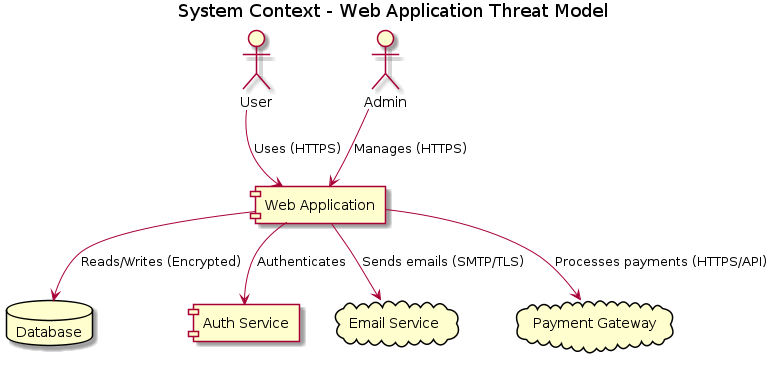
\includegraphics[width=0.7\textwidth]{images/system-context}
	\caption{Threat Modeling Workflow: From Asset Identification to Mitigation\cite{shostack2014}}
\end{figure}
